\documentclass{article} % Polska wersja klasy article

\usepackage{polski} % Pozwala na użycie polskiego. Ustawia między innymi fontenc na T1
\usepackage[utf8]{inputenc} % Informuje o kodowaniu
\usepackage{textcomp} % Znaki specjalne takie jak ~
\usepackage{xcolor} % Definicje kolorów
\usepackage{tcolorbox} % Ładne ramki

\renewcommand{\labelitemi}{\textbullet} % Zmiana symbolu wliczeń

\usepackage{graphicx}
\graphicspath{ {./Obrazy/} }
\usepackage{subcaption} % Subfigury
\usepackage{float} % Pozycjonowanie figur
\usepackage{mwe} % Tymczasowe grafiki

\usepackage{listings} % Listingi kodu
\lstset{basicstyle=\ttfamily,
  showstringspaces=false,
  commentstyle=\color{gray},
  keywordstyle=\color{blue},
  breaklines=true,
  frame=L,
  language=bash
}

\newcommand{\paragraphnl}[1]{\paragraph{#1} \mbox{} \\} % Paragraf z nową linią

\title{Laboratorium sieci komputerowych - c5 \\ Montowanie dysków sieciowych}
\author{Krzysztof Dąbrowski gr. 3}
\date{\today}

\begin{document}
\maketitle{}
\tableofcontents{}
%\newpage

\section{Cel zajęć}
Celem laboratorium c5 jest badanie udostępnionych dysków sieciowych i ich montowanie.
Przerabiane jest również instalowanie i konfiguracja serwerów SMB i NFS.

\section{Instalacja serwera SMB}
Chciałem uruchomić mój własny serwer SMB. W tym celu zainstalowałem serwer smb na stacji roboczej pod systemem Ubuntu.

\begin{verbatim}
  sudo apt install samba
\end{verbatim}

W celu sprawdzenie czy instalacja przebiegła pomyślnie skorzystałem z polecenia \texttt{whereis}.
\begin{verbatim}
  whereis samba

  samba: /usr/sbin/samba /usr/lib/samba /etc/samba /usr/share/samba /usr/share/man/man7/samba.7.gz /usr/share/man/man8/samba.8.gz
\end{verbatim}

Utworzyłem katalog, który będę udostępniał poleceniem \texttt{mkdir publicznyKatalog} oraz umieściłem w nim plik tekstowy.

\paragraph{Ustawienie konfiguracji} \mbox{} \\
Do pliku konfiguracyjnego dodałem ustawienie udostępniające katalog.

\begin{tcolorbox}[colback=yellow!10!white,colframe=red!45!black,coltitle=yellow!100!black, title=Konfiguracja serwera SMB]
  \begin{lstlisting}
  /etc/samba/smb.conf
  \end{lstlisting}
  \tcblower
  \footnotesize
  \begin{lstlisting}
  .
  .
  .

  [sambashare]
    comment = Samba na Ubuntu S6
    path = ~/publicznyKatalog
    read only = no
    browsable = yes 
  \end{lstlisting}
\end{tcolorbox}
\normalsize

\paragraph{Uruchomienie serwera SMB} \mbox{} \\
Uruchomiłem serwer SMB poleceniem \texttt{sudo service smbd restart}

By sprawdzić czy serwer działa wykonałem \texttt{sudo systemctl status smbd}
\begin{verbatim}
  sudo systemctl status smbd

  smbd.service - LSB: start Samba SMB/CIFS daemon (smbd)
   Loaded: loaded (/etc/init.d/smbd; bad; vendor preset: enabled)
   Active: active (running) since pon 2019-05-27 17:05:10 CEST; 11s ago
  ...
\end{verbatim}

Następnie ustawiłem hasło do zasobów serwera \texttt{sudo smbpasswd -a dabrowk1}

By sprawdzić czy zasób jest udostępniany uruchomiłem \texttt{smbclient -L s6}
\begin{verbatim}
  smbclient -L s6  

  WARNING: The "syslog" option is deprecated
  Enter dabrowk1's password: 
  Domain=[WORKGROUP] OS=[Windows 6.1] Server=[Samba 4.3.11-Ubuntu]

	Sharename       Type      Comment
	---------       ----      -------
	print$          Disk      Printer Drivers
	sambashare      Disk      Samba na Ubuntu S6
	IPC$            IPC       IPC Service (s6 server (Samba, Ubuntu))
	SK102           Printer   HP LaserJet M402dn
\end{verbatim}

\section{Windows}
Obsługę dysków sieciowych na systemie Windows wykonałem na maszynie Wat przy pomocy zdalnego pulpitu.

\subsection{SMB}

\subsubsection{Przeglądanie zasobów}
By zobaczyć zasoby udostępnione na stacji użyłem \texttt{net view s6}.

\begin{tcolorbox}[colback=yellow!10!white,colframe=red!45!black,coltitle=yellow!100!black, title=Windows]
  \begin{lstlisting}
  net view s6
  \end{lstlisting}
  \tcblower
  \footnotesize
  \begin{lstlisting}
  Shared resources at s6
  
  s6 server (Samba, Ubuntu)

  Share name  Type   Used as  Comment

  --------------------------------------------------------------
  sambashare  Disk            Samba na Ubuntu S6
  SK102       Print           HP LaserJet M402dn
  The command completed successfully.
  \end{lstlisting}
\end{tcolorbox}
\normalsize

\subsubsection{Montowanie zasobów}
Sprawdziłem zamontowane zasoby poleceniem \texttt{net use}.

\begin{tcolorbox}[colback=yellow!10!white,colframe=red!45!black,coltitle=yellow!100!black, title=Windows]
  \begin{lstlisting}
  net use
  \end{lstlisting}
  \tcblower
  \footnotesize
  \begin{lstlisting}
  New connections will not be remembered.


  Status       Local     Remote                    Network
  
  -----------------------------------------------------------
  OK           H:        \\stud\dabrowk1           Microsoft Windows Network
  The command completed successfully.
  \end{lstlisting}
\end{tcolorbox}
\normalsize
\vspace{5mm}

Następnie połączyłem dysk ze stacji \texttt{c6} poleceniem \texttt{net use :Z \textbackslash{}\textbackslash{}s6\textbackslash{}smbashare}.

By zobaczyć czy dysk jest zamontowany ponownie wykonałem \texttt{net use}.
\begin{tcolorbox}[colback=yellow!10!white,colframe=red!45!black,coltitle=yellow!100!black, title=Windows]
  \begin{lstlisting}
  net use
  \end{lstlisting}
  \tcblower
  \footnotesize
  \begin{lstlisting}
    New connections will not be remembered.


    Status       Local     Remote                    Network
    
    -----------------------------------------------------------
    OK           H:        \\stud\dabrowk1           Microsoft Windows Network
    OK           Z:        \\s6\sambashare           Microsoft Windows Network
    The command completed successfully.
  \end{lstlisting}
\end{tcolorbox}
\normalsize
\vspace{5mm}

By domontować dysk po zakończonej pracy wpisałem \texttt{net use Z: /delete}.

\subsection{NFS}

\subsubsection{Przeglądanie zasobów}
By zobaczyć zasoby nfs serwara volt uruchomiłem \texttt{showmount -e volt}.
\begin{tcolorbox}[colback=yellow!10!white,colframe=red!45!black,coltitle=yellow!100!black, title=Windows]
  \begin{lstlisting}
  showmount -e volt
  \end{lstlisting}
  \tcblower
  \footnotesize
  \begin{lstlisting}
    Exports list on volt:
    /tmp/obj                           All Machines
    /home/stud                         ldap, fed.iem.pw.edu.pl, ...
    /nfs                               lap
  \end{lstlisting}
\end{tcolorbox}
\normalsize

\subsubsection{Montowanie zasobów}
By zamontować katalog udostępniany przez serwer wykonałem \texttt{mount \\volt\ I:}
\begin{tcolorbox}[colback=yellow!10!white,colframe=red!45!black,coltitle=yellow!100!black, title=Windows]
  \begin{lstlisting}
  mount \\volt\ I:
  \end{lstlisting}
  \tcblower
  \footnotesize
  \begin{lstlisting}
  I: is now successfully connected to \\volt\

  The command completed successfully.
  \end{lstlisting}
\end{tcolorbox}
\normalsize
\vspace{5mm}

By sprawdzić czy zasób jest poprawnie zamontowany wykonałem \texttt{mount} bez argumentów.
\begin{tcolorbox}[colback=yellow!10!white,colframe=red!45!black,coltitle=yellow!100!black, title=Windows]
  \begin{lstlisting}
  mount
  \end{lstlisting}
  \tcblower
  \footnotesize
  \begin{lstlisting}
  Local    Remote
  ----------------
  I:       \\volt\
  \end{lstlisting}
\end{tcolorbox}
\normalsize
\vspace{5mm}

Na koniec odłączyłem dysk poleceniem \texttt{umount I:}.

\section{Ubuntu}
Ćwiczenie wykonałem na stacji laboratoryjne c6, na której wcześniej postawiłem serwer SMB.

\subsection{SMB}

\subsubsection{Przeglądanie zasobów}
W celu zobaczenia zasobów na stacji uruchomiłem \texttt{smbclient -L s6}
\begin{tcolorbox}[colback=yellow!10!white,colframe=red!45!black,coltitle=yellow!100!black, title=Ubuntu]
  \begin{lstlisting}
    smbclient -L s6
  \end{lstlisting}
  \tcblower
  \footnotesize
  \begin{lstlisting}
    Sharename       Type      Comment
    ---------       ----      -------
    print$          Disk      Printer Drivers
    sambashare      Disk      Samba na Ubuntu S6
    SK102           Printer   HP LaserJet M402dn
  \end{lstlisting}
\end{tcolorbox}
\normalsize

\subsubsection{Montowanie zasobów}
Zamontowałem utworzony wcześniej zasób poleceniem \texttt{sudo mount -t cifs -o user=dabrowk1 //s6/sambashare punktMontowania}.

W celu sprawdzenia poprawności montowania spróbowałem wypisać zawartość zamontowanego katalogu.
\begin{tcolorbox}[colback=yellow!10!white,colframe=red!45!black,coltitle=yellow!100!black, title=Ubuntu]
  \begin{lstlisting}
  ls punktMontowania
  \end{lstlisting}
  \tcblower
  \footnotesize
  \begin{lstlisting}
  plik1.txt
  \end{lstlisting}
\end{tcolorbox}
\normalsize

\subsection{NFS}

\subsubsection{Przeglądanie zasobów}
W celu zobaczenia zasobów udostępnianych przez serwer ldap użyłem polecenia \texttt{showmount}.
\begin{tcolorbox}[colback=yellow!10!white,colframe=red!45!black,coltitle=yellow!100!black, title=Ubuntu]
  \begin{lstlisting}
    showmount -e ldap
  \end{lstlisting}
  \tcblower
  \footnotesize
  \begin{lstlisting}
  Export list for ldap:
  /home/stud2 (everyone)
  /nfs/arch2  k0.iem.pw.edu.pl,pxe.iem.pw.edu.pl,s2.iem.pw.edu.pl
  /           (everyone)
  \end{lstlisting}
\end{tcolorbox}
\normalsize

\subsection{Montowanie zasobów}
Zamontowałem katalog / z serwera poleceniem \texttt{sudo mount -t nfs ldap:/ mountingPoint}.

W celu testu poprawności montowania spróbowałem wypisać zawartość katalogu.
\begin{tcolorbox}[colback=yellow!10!white,colframe=red!45!black,coltitle=yellow!100!black, title=Ubuntu]
  \begin{lstlisting}
  ll mountingPoint
  \end{lstlisting}
  \tcblower
  \footnotesize
  \begin{lstlisting}
  lrwxr-xr-x  1 root root    21 gru  9 03:32 10
  lrwxr-xr-x  1 root root    20 gru  6  2018 11
  lrwxr-xr-x  1 root root    20 lut  3  2018 12
  lrwxr-xr-x  1 root root    20 paz 23  2018 13
  -rw-r--r--  1 root root 1000M kwi 15 20:07 1G 
  -rw-r--r--  1 root root  2,0G kwi 15 20:12 2G
  drwxr-xr-x  2 root root    47 cze  9 17:31 bin
  ...
  \end{lstlisting}
\end{tcolorbox}
\normalsize
\vspace{5mm}

Na koniec odmontowałem zasób poleceniem \texttt{sudo umount mountingPoint}.

\section{FreeBSD}
Realizowałem zadanie zdalnie na stacji \texttt{se}.

\subsection{SMB}

\subsubsection{Przeglądanie zasobów}
Sprawdziłem dyski SMB eksportuje serwer \texttt{volt} poleceniem \texttt{showmount}.

\begin{tcolorbox}[colback=yellow!10!white,colframe=red!45!black,coltitle=yellow!100!black, title=FreeBSD]
  \begin{lstlisting}
  showmount -e volt -t cifs
  \end{lstlisting}
  \tcblower
  \tiny
  \begin{lstlisting}
    Exports list on volt:
  /tmp/obj                           Everyone
  /home/stud                         ldap fed.iem.pw.edu.pl ...
  /                                  Everyone
  /nfs                               lap
  \end{lstlisting}
\end{tcolorbox}
\normalsize

\subsubsection{Montowanie zasobów}
Utworzyłem katalog będący punktem montowania poleceniem \texttt{mkdir mountingPoint}

Zamontowałem katalog z serwera volt poleceniem \texttt{mount\_smbfs -I volt -U dabrowk1 //dabrowk1@volt/lok mountingPoint/}.

By sprawdzić poprawność montowania wypisałem zawartość katalogu.
\begin{tcolorbox}[colback=yellow!10!white,colframe=red!45!black,coltitle=yellow!100!black, title=FreeBSD]
  \begin{lstlisting}
  ll mountingPoint
  \end{lstlisting}
  \tcblower
  \tiny
  \begin{lstlisting}
  drwxr-xr-x  1 root  wheel  16384 Feb  9  2014 backups 
  drwxr-xr-x  1 root  wheel  16384 Dec 16  2015 e0
  drwxr-xr-x  1 root  wheel  16384 Oct  6  2014 www
  \end{lstlisting}
\end{tcolorbox}
\normalsize
\vspace{5mm}

Na koniec odmontowałem katalog poleceniem \texttt{umount mountingPoint}.

\subsection{NFS}

\subsubsection{Przeglądanie zasobów}
Sprawdziłem jakie dyski NFS eksportuje serwer \texttt{ldap}.
\begin{tcolorbox}[colback=yellow!10!white,colframe=red!45!black,coltitle=yellow!100!black, title=FreeBSD]
  \begin{lstlisting}
  showmount -e ldap -t nfs
  \end{lstlisting}
  \tcblower
  \tiny
  \begin{lstlisting}
    Exports list on ldap:
    /                                  Everyone
    /nfs/arch2                         s2.iem.pw.edu.pl pxe.iem.pw.edu.pl k0.iem.pw.edu.pl  
    /home/stud2                        Everyone
  \end{lstlisting}
\end{tcolorbox}
\normalsize

\subsubsection{Montowanie zasobów}
Zamontowałem dysk poleceniem \texttt{mount -t nfs ldap:/ mountingPoint}. Następnie sprawdziłem czy dysk jest zamontowany poleceniem \texttt{df -h}.

Dla odmiany sprawdziłem czy katalog jest zamontowany poleceniem \texttt{df -h}.
\begin{tcolorbox}[colback=yellow!10!white,colframe=red!45!black,coltitle=yellow!100!black, title=FreeBSD]
  \begin{lstlisting}
  df -h
  \end{lstlisting}
  \tcblower
  \tiny
  \begin{lstlisting}
    Filesystem    Size    Used   Avail Capacity  Mounted on
    /dev/md0      274M    147M    105M    58%    /
    devfs         1.0K    1.0K      0B   100%    /dev
    tmpfs         2.3G     16K    2.3G     0%    /tmp
    tmpfs         2.3G     12M    2.3G     1%    /var
    ldap:/R        58G     30G     27G    53%    /net/ldap
    ldap:/         58G     30G     27G    53%    /root/mountingPoint 
  \end{lstlisting}
\end{tcolorbox}
\normalsize

Następnie odmontowałem dysk poleceniem \texttt{umount mountingPoint}.

\section{Implementacja dowolnego serwera i klienta w środowisku wirtualnym}
Ponieważ na laboratoriach instalowałem już serwer SMB postanowiłem to powtórzyć.

\subsection{Diagram sieci}
\begin{figure}[h]
  \caption{Diagram sieci}
  \centering
  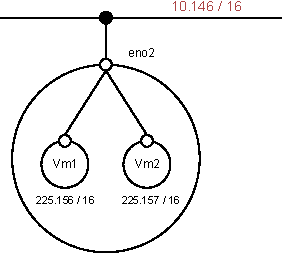
\includegraphics[width=0.5\textwidth]{Schemat_sieci}
\end{figure}

\subsection{Generacja maszyn}
Skrypty generujący maszyny

\lstinputlisting[caption={install-vm.sh}]{./Skrypty/install-vm.sh}
\lstinputlisting[caption={Tworzenie maszyn}]{./Skrypty/tworzenie-maszyn-c5.sh}

\section{Konfiguracja serwera}
Na maszynie musiałem utworzyć zasób od udostępniania, zainstalować serwer SMB oraz skonfigurować i uruchomić serwer.

\lstinputlisting[caption={Konfiguracja serwera}]{./Skrypty/instalacja-smb.sh}

\section{Konfiguracja klienta}
\lstinputlisting[caption={Konfiguracja klienta}]{./Skrypty/konfiguracja-klienta.sh}

\end{document}